\chapter{Analysis}
\label{chap:analysis}

\section{General vs. domain specific solution}
We have chosen to implement the application solely for ITU, to include support for domain specific constraints and situations. The semester planning part of our application is not a trivial problem to solve. It fact, it is a so called NP-problem, which is a problem that is unsolvable within a reasonable period of time. This is due to the many types of constraints, which can vary a lot for each domain. While we concentrate on the UI and not the algorithms that should actually solve the problem, we still need to provide the data nessesary for the algorithm to function.\\
By making it a domain specific problem, we can limit the number of constraints to reduce the complexity. This makes it possible for us to include only the relevant user interface elements, and exclude the elements that \emph{might} have been relevant for other domains. This reduces clutter of the interface, and makes it possible for us to include support for the needed domain specific elements.

\section{Existing solutions}
\label{sec:existing_solutions}
Existing solutions can be divided into two categories:

\begin{itemize}
	\item \textbf{Room management software}\\
This kind of software gives a good visualization of available rooms on a current day. All programs have taken a general approach by listing each room on the x-axis, time on the y-axis and boxes representing a reservation with information inside it. Figure \ref{fig:app1} shows an example of such an application.\\

\begin{figure}[htb]
\begin{center}
\leavevmode
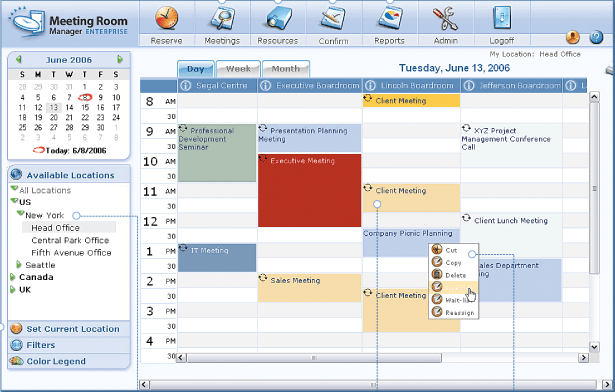
\includegraphics[width=0.6\textwidth]{images/app1.png}
\end{center}
\caption{Meeting Room Manager by NetSimplicity \cite{meeting_room_manager}}
\label{fig:app1}
\end{figure}

While having nothing to do with semester planning, this representation works as a room booking system if you only have a few rooms. On a 800x600 resolution monitor, 5 rooms is enough to make horizontal scroll nessesary, making it hard to get an good overview of the current occupation of the rooms.

\item \textbf{Schema based planning software}\\
These applications are developed for primary schools and universities. They show weekdays on the the x-axis, time on the y-axis and a box in the schema represents a booked time slot. This gives a good weekly overview, but you cannot get an overview of how a specific room is used. More importantly, ITU needs another abstraction level, the tracks, representing one semester for a particular study programme, which is not possible to represent in any of the applications. This would make it hard to gather information from a particular track, as the related courses would be scattered throughout the overview. Figure \ref{fig:app2} shows an example of a schema planning application.
\end{itemize}

\begin{figure}[htb]
\begin{center}
\leavevmode
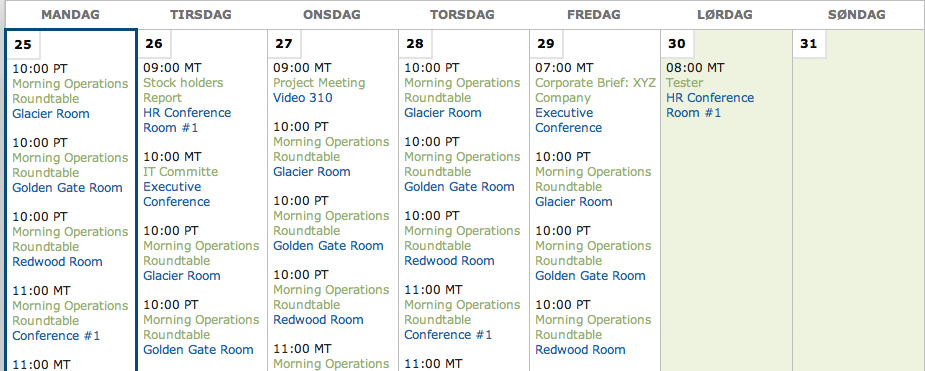
\includegraphics[width=0.6\textwidth]{images/app2.png}
\end{center}
\caption{EMS Campus by DEA \cite{ems_campus}}
\label{fig:app2}
\end{figure}

In general, all of the applications take a general approach. This makes the user interface less user friendly, as important application specific variables cannot be taken into account, like a map of the specific building or domain specific naming conventions.

\section{Target audience} % (fold)
\label{sec:target_audience}
Our target audience can be divided into two groups:
\begin{itemize}
\item Student body at ITU
\item Employees at ITU
\end{itemize}

\subsection*{Student body}
The student body covers ages 18 - 40+ and with very different backgrounds. Based on the nature of the university, it is fair to assume that most students have at least basic familiarity with IT and computer use in general.

\subsection*{Employees}
The computer proficiency of the employees can range from expert to novice, and no clear-cut distinctions can be made. We have, however, observed that the majority of the people our system would affect are using tools with some similarities, and are therefore assuming their proficiency to be above novice users.\\

Note that even though our day to day booking interface will mostly be used by students, we can make no assumptions that the target audience for this part of the application \emph{only} contains students. We need to make sure the day to day booking can be used by a very wide range of people, including also the employees.\\
No one outside of ITU (not being registrered in the userbase) should be able to use the application, as it should not be possible for random companies to book and occupy rooms without permission.

\section{Requirements}
\label{sec:requirements}
% L�s s�ren la om Requirements
Since the ITU does not currently have a full system, we have put up initial requirements for such a system.
As described in the target audience \ref{sec:target_audience}, the system will be used by a wide variety of people, and there will be virtually no way to train them. We have met this problem by writing up all the tasks our system must support, along with quality requirements describing success criterias for our application. \cite{lauesen}

\subsection{Non-functional requirements} % (fold)
\label{subsec:non_functional_requirements}
Preparing for the creation of mockups following various usability tests, it is nessesary to set up a reference point to what we actually want to measure. This helps us to keep the following mockups and usability tests focused.\\
Usability quickly becomes very subjective, if you do not attempt to define it in more precise terms. We have used Soren Lausens five usability requirements \cite{lauesen}, as a measurement of the usability of our application.\\

In a perfect world, one might think that all of the 5 usability requirements would be met. However, this is rarely desired, as it does not emulate a clear focus of what should be prioritised in the application. Here follows a rundown of the usability factors and how they relate to our project. Note that the \textbf{fit for use} requirement has been left out. This is defined as:\\

\emph{Can the system support the tasks that the user has in real life?}\\

We do not think this is an actual usability requirement, as it is merely concerned with the functionality of the program.
\begin{itemize}
	\item \textbf{Task efficiency}\\
	Since the task of finding a room often will be done on the fly, on the way to school, or right before a meeting takes place, it is important that the application is responsive and gives the user a proper response to a booking query. It should give the user a good overview to support his decision, and suggest alternatives if his query cannot be met. In general, we have failed if the user finds it more effective to book a room the old fashioned way, by asking the Facility Management.
	\item \textbf{Understandability}\\
	Interviewing the Study Administration suggested that the staff responsible for doing the semester planning had a large need to double-check that the important tasks performed by the system were done correctly. \ref{app:interview}. In general, they had very little confidence in the system. Therefore, to avoid resistance towards change, it is important that the system clearly communicates it's functionality to the user, during normal use, and expecially in error prone situations to avoid confusion.
	\item \textbf{Ease of learning}\\
	The set of people using our system is large and will change rapidly. It is therefore important that the system can be used "out of the box". If not, people will simply not use it, as it takes to much of their already limited time to get familiar with. Also, there is a close relation between ease of learning, and the effectiveness of the support the system offers. If the user does not understand how to use the system, they will not be able to benefit from the support layer.
	\item \textbf{Subjective satisfaction}\\
	Some might argue that the subjective satisfaction is not very relevant in our case, because we're developing a tool for daily support and not a program that in any way should be amusing or entertaining. \\
However experts believe that users are more willing to accept the program and trust its efficiency if they find it visually appealing\cite{nielsen_metrics}. Apple is a good example of using design and pleasing aesthetics as major selling points. The iPad used this to brand itself, thus creating a need that in reality was not present. %Source?
\end{itemize}

\subsection{Functional requirements}
\label{subsec:functional_requirements}
To establish a foundation for the requirements of our system, we have considered the functionality our system must contain. These functional requirements only contains high level goals, and not \emph{how} they must be met, as we will adjust the way they take place based on usability factors.

The system must... \begin{enumerate}
\item distinguish users from each other
\item store data and information persistently
\item support the user in performing the tasks specified in section \ref{sec:tasks}
\end{enumerate}

In regard to the first item, all students and faculty at the ITU already have unique logins, and it would be natural to reuse those for our system. Also, it should not be possible for non-authorized users to use our system. Being a webbased system, it comes as no surprise that we wish the data to be stored persistantly so different computers at different times can be used, without the loss of bookings or the like.
Naturally, the system has no use without actually fulfilling the tasks it has been designed to, hence the listing as a functional requirement.\\

Note that we have few functional requirements compared to some systems. This stems from the fact that the system, from an end-user perspective, is pretty simple. Our vision is simply to enforce this perspective, and provide the \emph{expected} functionality, without hindrance of high complexity and feature creep. \cite{porter}

\section{Tasks}
\label{sec:tasks}
The following tasks are the actions able to be performed within our system.

\begin{itemize}\itemsep1pt
\item[\textbf{1.}] \textbf{Day-to-day booking}
\item[\textbf{T1.1}] Book room. May or may not be a specific room or a specific time/day
\item[\textbf{T1.2}] Check availability of room. May or may not be today.
\item[\textbf{T1.3}] Cancel booking. May or may not be before the booked timeslot.
\item[\textbf{T1.4}] Extend booking. May or may not be before the booked timeslot.
\\
\item[\textbf{2.}] \textbf{Semester planning}
\item[\textbf{T2.1}] Create course. May or may not have full information available at the point of creation.
\item[\textbf{T2.2}] Create track.
\item[\textbf{T2.3}] Edit course.
\item[\textbf{T2.4}] Edit track.
\item[\textbf{T2.5}] Plan semester. A full solution may or may not be possible
\end{itemize}

A full example task including subtasks can be found below, while the full list including subtasks covering all scenarios can be found in appendix \ref{app:tasks}.

\begin{tabular}{|p{6cm}|p{6cm}|}
\hline 
	\multicolumn{2}{|l|}{\textbf{T1.1:} \hspace{26mm}Book room} \\
	\multicolumn{2}{|l|}{Start: \hspace{26mm}User opens system } \\
	\multicolumn{2}{|l|}{End: \hspace{28mm}User have gotten a room } \\
	\multicolumn{2}{|l|}{Frequency: \hspace{17mm}Average of 10 bookings pr. day} \\
	\multicolumn{2}{|l|}{Difficult when: \hspace{10mm}No rooms are available } \\ \hline
	\multicolumn{1}{|c|}{\textbf{Subtasks}} & \multicolumn{1}{c|}{\textbf{Example solution}} \\ \hline
	1.  Find room & \\
	1a. No specific room needed & System suggests any available room\\
	1b. User has specific needs & System allows to search by parameters\\
	1c. No available rooms & System allows to search at future dates\\ \hline
	2.  Book room & \\
	2a. User does not specify booking duration & System suggests a standard time duration \\
	2b. User specifies time interval & \\ \hline
	3. Confirm booking & \\
	3a. User confirms & \\
	3b. User declines & System cancels the booking \\ \hline
\end{tabular}

\subsection{Quality Requirements}
\label{subsec:quality_requirements}
Based on the task list above, we can finally put forth the list of quality requirements we wish to meet in able to consider the level of usability acceptable.
\begin{enumerate}\itemsep1pt
\item Without instructions, 90\% of novice users must be able to complete T1.1 to T1.4 without variants.
\item Without instructions, 80\% of novice users must be able to complete T1.1 to T1.4 including variants.
\item With a maximum of 30 minutes instructions, 90\% of administration personel must be able to complete T2.1 to T2.5.
\item Without instructions, 50\% administration personel must be able to complete T2.1 to T2.5.
\end{enumerate}

\section{Domain specific challenges}
\label{sec:domain_challenges}
Throughout the project, we encountered some very domain specific challenges, that ultimately should be answered by ITU. They are nevertheless important to our application and will be highlighted in this section. We have discussed these issues with a member of the study administration, and our default choices are based on that, but it is something that ITU as an institution must decide on policies for.

\subsection{Approval}
\label{subsec:approval}
It is very plausible that FM wishes to assume full control of the rooms. In practice, this would mean that users could make requests for rooms, and FM would then manually have to approve or decline every request. We find it a very reasonable wish, but with a caveat: If FM is not constantly active, it would not be a big improvement over the current way of handling rooms, but simply a new look to an old way. In our prototype, we have assumed that FM would be willing to accept the users making bookings themselves, and simply grant them the power to delete bookings at will.

\subsection{Limiting bookings}
\label{subsec:limiting_bookings}
To prevent abuse, such as a student booking the whole school for a month straight, it is important to have some limitations based on user levels. For example, limiting a student to have one or two active bookings, and possibly more for staff and faculty. This would of course already be solved if the aforementioned approval system was agreed upon.

\subsection{Overriding bookings}
\label{subsec:overriding_bookings}
We mention  in section \ref{subsec:relations} that semester planning should take precedency over day to day booking, and that it might not always be the case in reality. This is a policy that ITU internally have to sort out, and we will have to adjust the application according to their final decision. By default, we will however allow day to day bookings to be overwritten, as it is our belief that a good room allocation is more important than a single meeting/appointment. \\
\\
Another concern regarding prioritizing bookings, are the cases of extending bookings. If a users wishes to extend a booking for a room they currently occupy, and another booking has been made already, it could be considered if the current occupant should be allowed to extend if a replacement room can be found automatically for the secondary booking. By default however, extending is only possible if the room is not booked.

\subsection{Occupation of rooms without booking}
\label{subsec:occupation}
If a user books a room that according to our system is available, but in reality is occupied, ownership of the room can become a point of argument. One would think that the day to day booking functionality is there to make it easier for people to book rooms, but still being an optional tool to use if you find it useful. \\
This might not be possible in reality though, because of situations like the before mentioned. We therefore assume that rooms should be booked before you have the right to use them. This is a very important point, as this will force some people to use the program, ever though they dont want to. The program should thus be very easy and quick to use, so the users dont feel they waste time booking a room, when they could have just avoided it. 



